\documentclass[11pt]{beamer}

\usetheme{metropolis}

\usepackage{graphicx}
\usepackage{physics}
\usepackage{adjustbox}
\usepackage{caption}
\usepackage{chemformula}
\usepackage{quoting}
\usepackage[style=chem-angew,backend=bibtex]{biblatex}
\bibliography{references}
%
% Choose how your presentation looks.
%
% For more themes, color themes and font themes, see:
% http://deic.uab.es/~iblanes/beamer_gallery/index_by_theme.html
%
\mode<presentation>
{
  \usetheme{default}      % or try Darmstadt, Madrid, Warsaw, ...
  \usecolortheme{default} % or try albatross, beaver, crane, ...
  \usefonttheme{default}  % or try serif, structurebold, ...
  \setbeamertemplate{navigation symbols}{}
  \setbeamertemplate{caption}[numbered]
  \setbeamerfont{footnote}{size=\tiny}
} 

\usepackage[english]{babel}
\usepackage[utf8]{inputenc}
\graphicspath{{../lectureMW/image/}}

\AtBeginSection[]{
\begin{frame}{Outline}
  \tableofcontents[currentsection]
\end{frame}
}

\title{Chapter 3: Chemical Compounds}
\institute{Chemistry Department, Cypress College}
\date{Sept 13, 2022}

\begin{document}

\begin{frame}
  \titlepage
\end{frame}

\begin{frame}{Class Announcements}
  \begin{itemize}
  \item Go over homework assignment; present your work
    for 1pt EC
  \item Begin Ch 3 - Chemical Compounds and Types of Bonding
  \item Quiz \#3 released this Fri, Sept 16 at 3pm and due Tues,
    Sept 20 at 11:59pm
  \item Homework \#3 released this Fri, Sept 16 at 3pm and due
    Fri, Sept 23 at 11:59pm
  \end{itemize}  
\end{frame}

\begin{frame}{Lecture Weekly Agenda}

  \begin{itemize}
  \item Go over homework assignment; present your work
    for 1pt EC
  \item Review Ch 2 - Atoms, Ions, and the Periodic Table
  \item Begin lecture on Ch 3 - Chemical Compounds and
    Nomeclature
  \item Nomenclature Lab assignments due Sept 19 at 11:59pm
  \end{itemize}
\end{frame}

\section{Review: Chapter 2 Highlights}

\begin{frame}{J.J. Thompson's Plum Pudding Model}
  \centering
  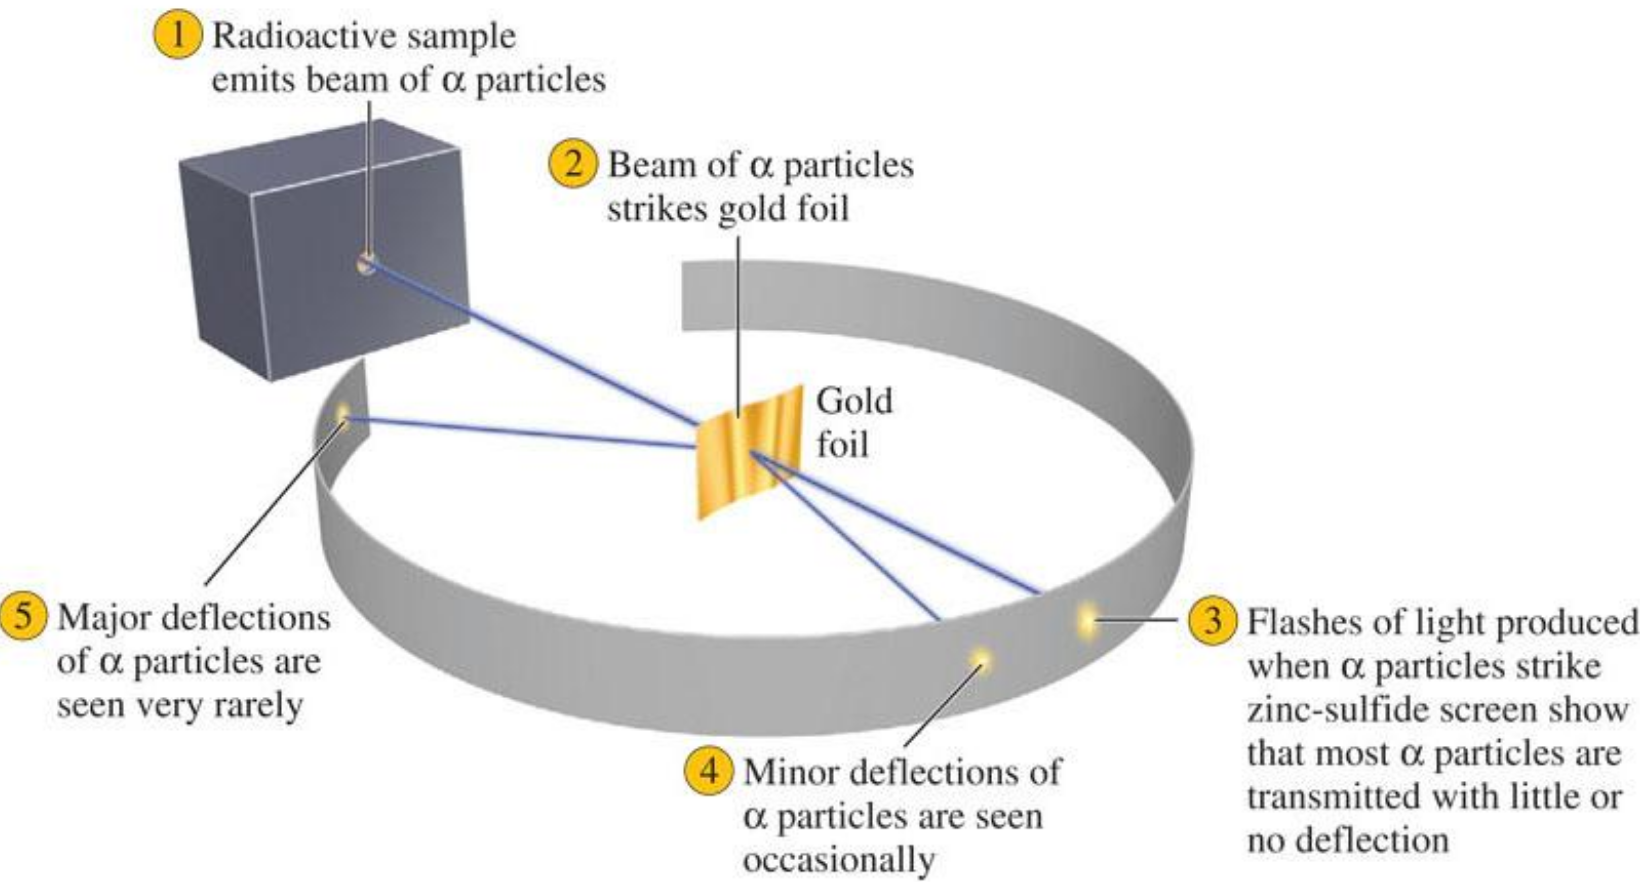
\includegraphics[scale=0.175]{alpha}
\end{frame}

\begin{frame}{Review: Modern Period Table}
  \centering
  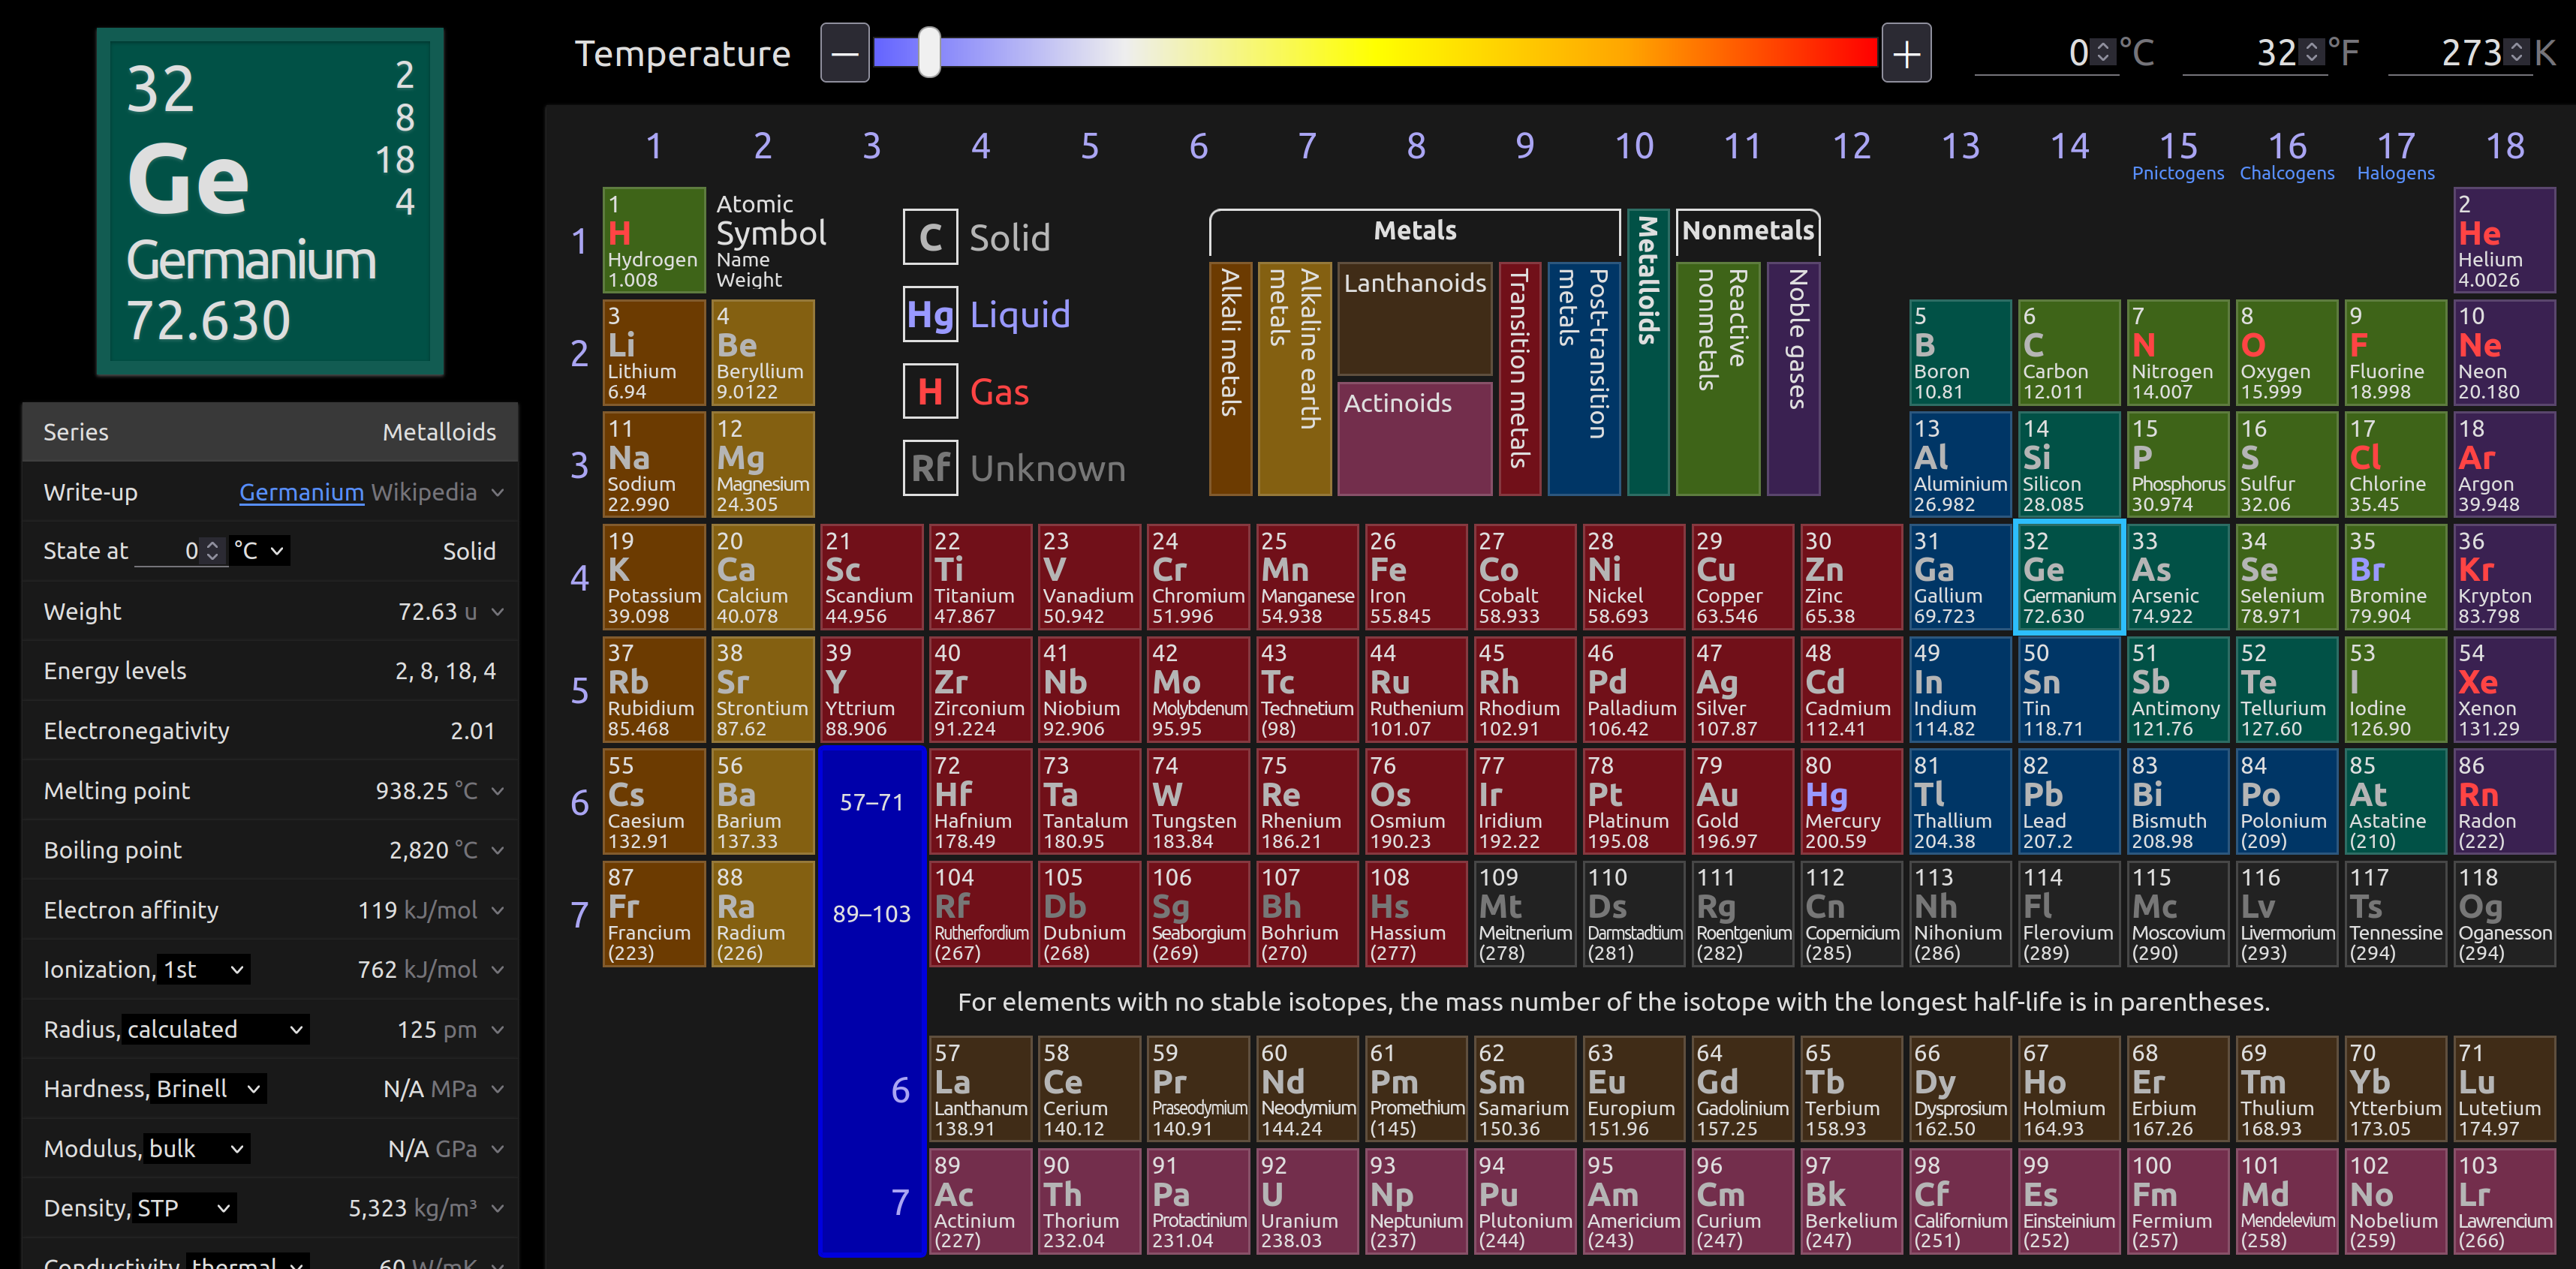
\includegraphics[width=\linewidth]{ptable}
\end{frame}

\begin{frame}{Relative Atomic Mass}
  \begin{equation}
    \text{Relative Atomic Mass} = (I_1\times A_1) + (I_2\times A_2) + \dots
  \end{equation}
  where $I$ is the mass of the isotope, and $A$ is the
  relative abundance between 0 and 1
\end{frame}

\begin{frame}{Defining Atomic Number and Mass}
  \begin{equation}
    ^\text{A}_\text{Z}\text{X}^\text{C}
  \end{equation}

  where A is the atomic mass, Z is the atomic number, X is atomic
  symbol, and C is the overall charge

  \textbf{Isotopes} - chemically same atom (same number of protons)
  but physically different (different number of neutrons)
\end{frame}

\begin{frame}{Hydrogen Isotopes and Applications}
  \begin{center}
    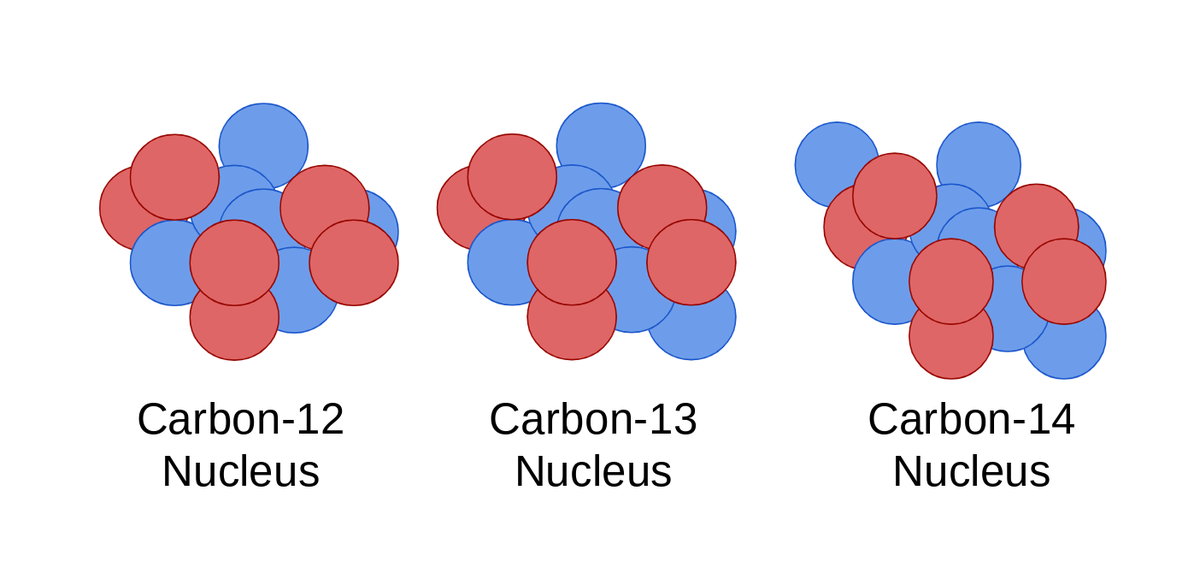
\includegraphics[width=0.75\linewidth]{carbon_isotopes}
  \end{center}

  \begin{itemize}
  \item Carbon-12, carbon-13, and carbon-14
    have relative abundances of $98.9\%$, $1.1\%$, and $0.1\%$,
    respectively
  \item \textbf{Q:} Which carbon isostope is the highest in abundance?
  \end{itemize}
\end{frame}

\begin{frame}{Carbon-14 Dating}
  \begin{center}
    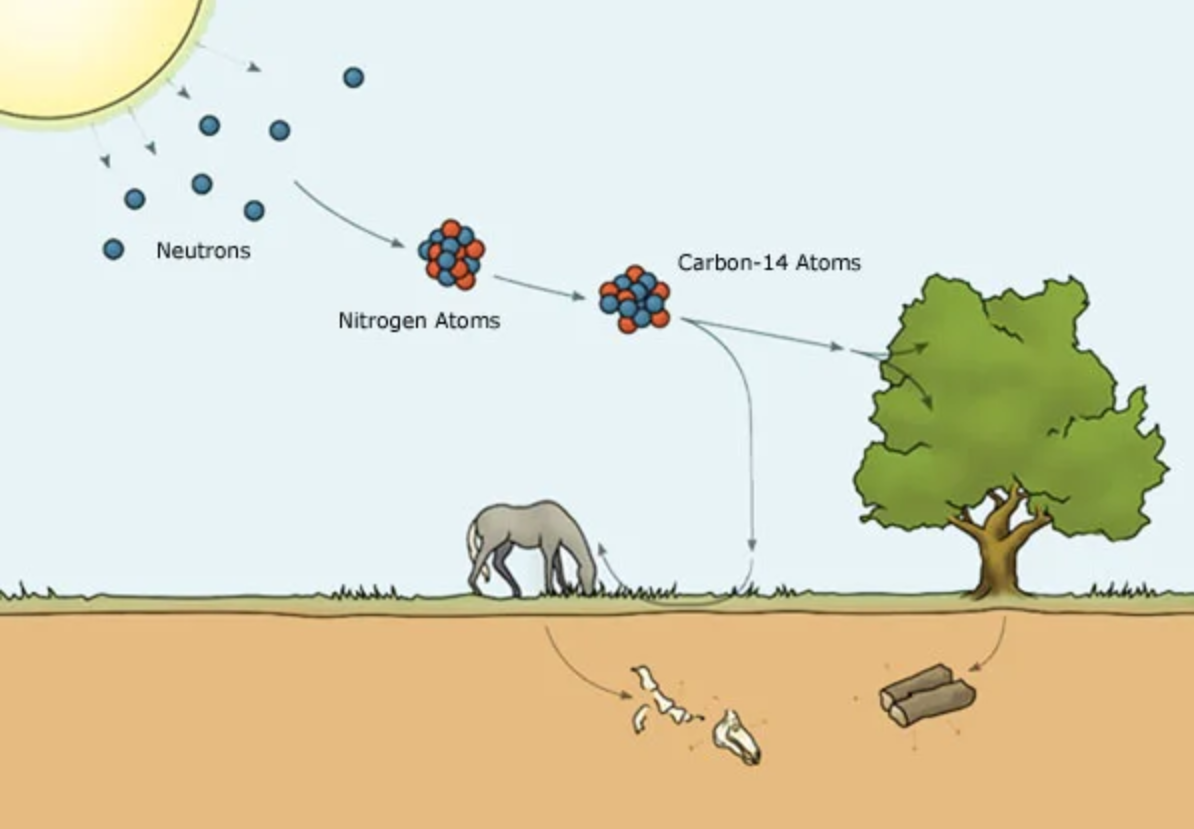
\includegraphics[width=0.75\linewidth]{carbon_14_dating}
  \end{center}

  \textbf{Applications}
  
  \begin{itemize}
  \item Rough estimation of fossils because known half-life $\sim 5,730$ years
  \end{itemize}
\end{frame}

\begin{frame}{Experiment: Mass Spectroscopy}
  \begin{center}
    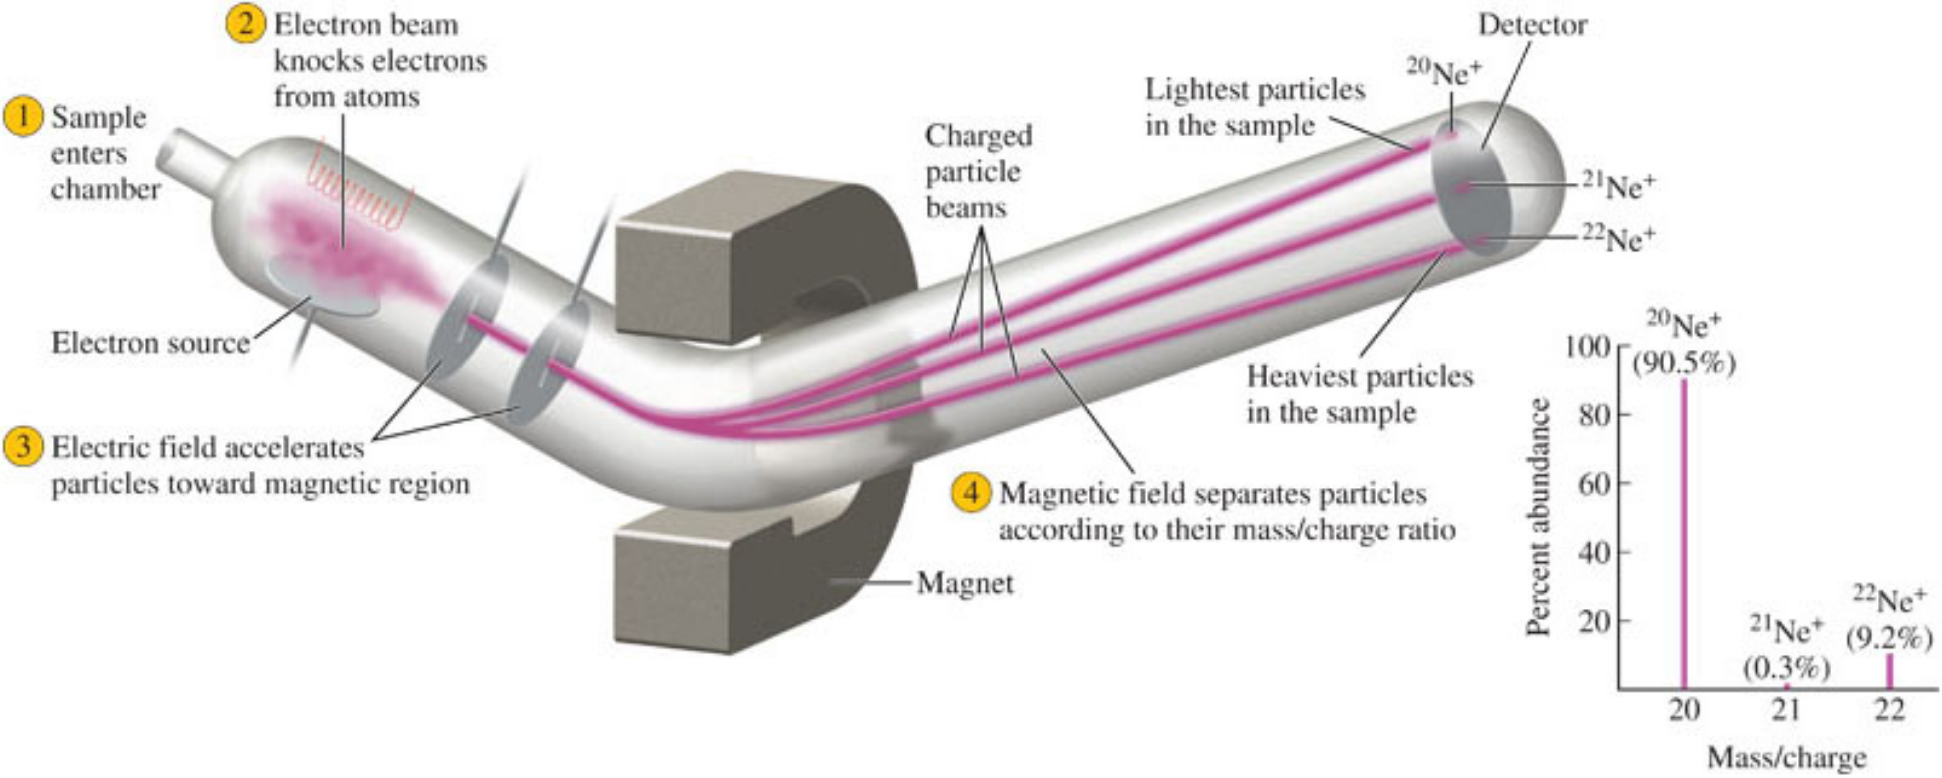
\includegraphics[width=\linewidth]{mass_spect}
  \end{center}

  \begin{itemize}
  \item Ionizes the atom and electric field accelerates atoms
  \item Time of flight - heavier atoms will travel slower
    than lighter ones
  \item Weighted average of atomic masses
  \end{itemize}  
\end{frame}

\section{Ionic and Molecular Compounds}

\begin{frame}{Ionic and Molecular Compounds}
  \textbf{Ionic Compounds}
  \begin{itemize}
  \item Consists of oppositely charged cations and anions
    such that the overall charge is neutral e.g CaCl$_2$(s),
    BaF(s), and Fe$_2$O$_3$(s)
  \item Electrolyte - substances that separate into the ions
    e.g. NaCl(aq) dissociates into Na$^+$ and Cl$^-$
  \item Forms ionic bonds (purely electrostatic interactions)
  \end{itemize}

  \textbf{Molecular Compounds}
  \begin{itemize}
  \item Composed of atoms from two or more nonmetals
  \item Forms covalent bonds (sharing of electrons)
  \end{itemize}
\end{frame}

\begin{frame}{Properties of Ionic and Molecular Compounds}
  \begin{center}
    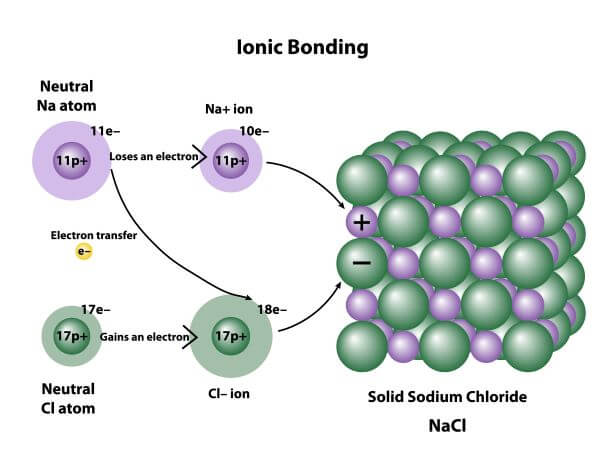
\includegraphics[width=0.6\linewidth]{Ionic-bond-example}
  \end{center}
  \vspace{-0.3in}
  \textbf{Ionic Compounds}
  \begin{itemize}
  \item Highly conductive and strong electrolyte - ability to
    carry electricity (electrons)
  \item High melting and boiling points, high density
  \end{itemize}
\end{frame}

\begin{frame}{Properties of Ionic and Molecular Compounds}
  \begin{center}
    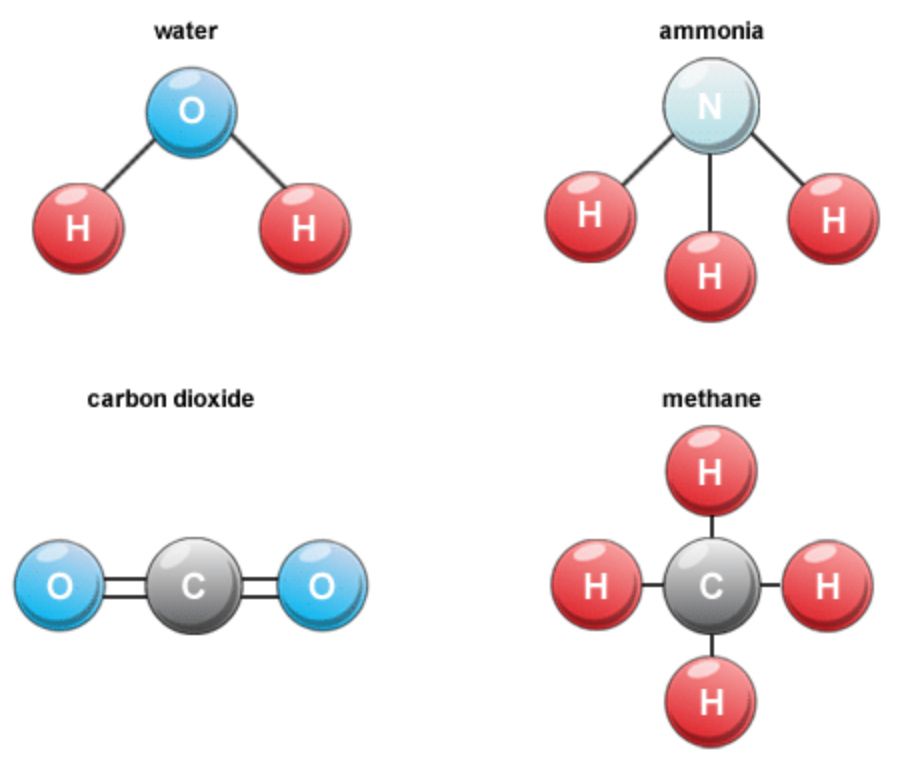
\includegraphics[width=0.6\linewidth]{molec_example}
  \end{center}
  \vspace{-0.3in}
  \textbf{Molecular Compounds}
  \begin{itemize}
  \item Not conductive and weak electrolyte
  \item Low melting and boiling points, low density
  \end{itemize}
\end{frame}

\subsection{Monoatomic and Polyatomic Ions}

\begin{frame}{Monoatomic Ions}
  \centering
  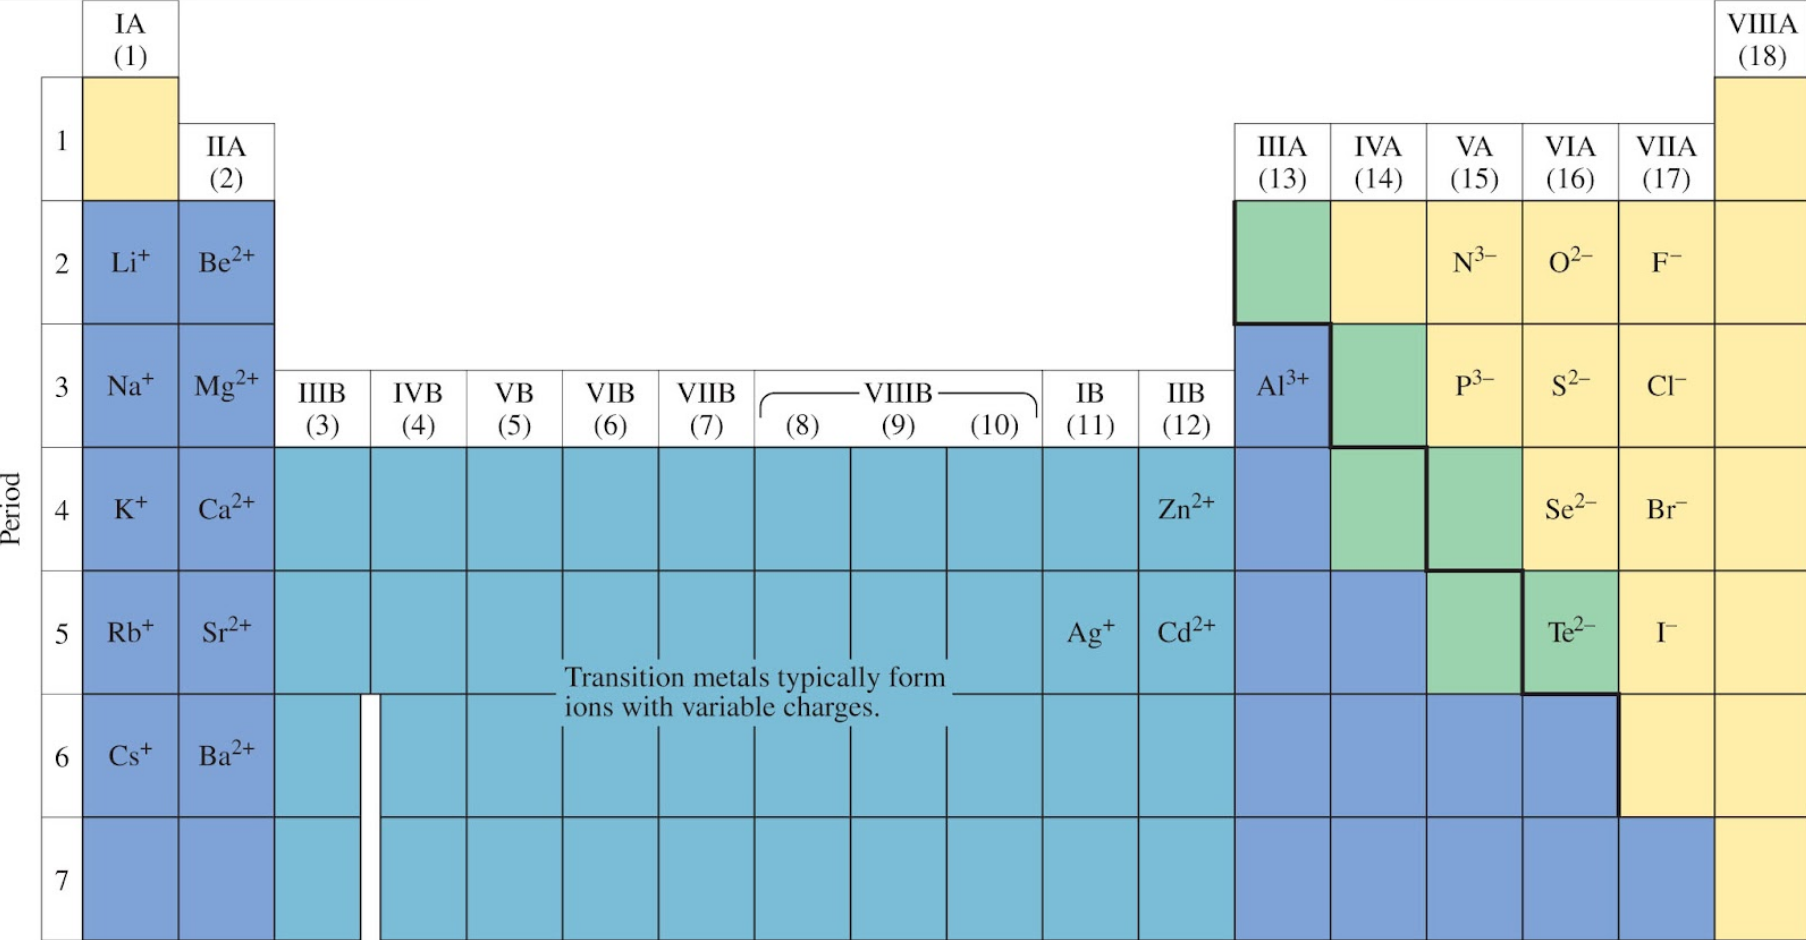
\includegraphics[width=\linewidth]{monoatomic_ion}
\end{frame}

\begin{frame}{Polyatomic Ions}
  \centering
  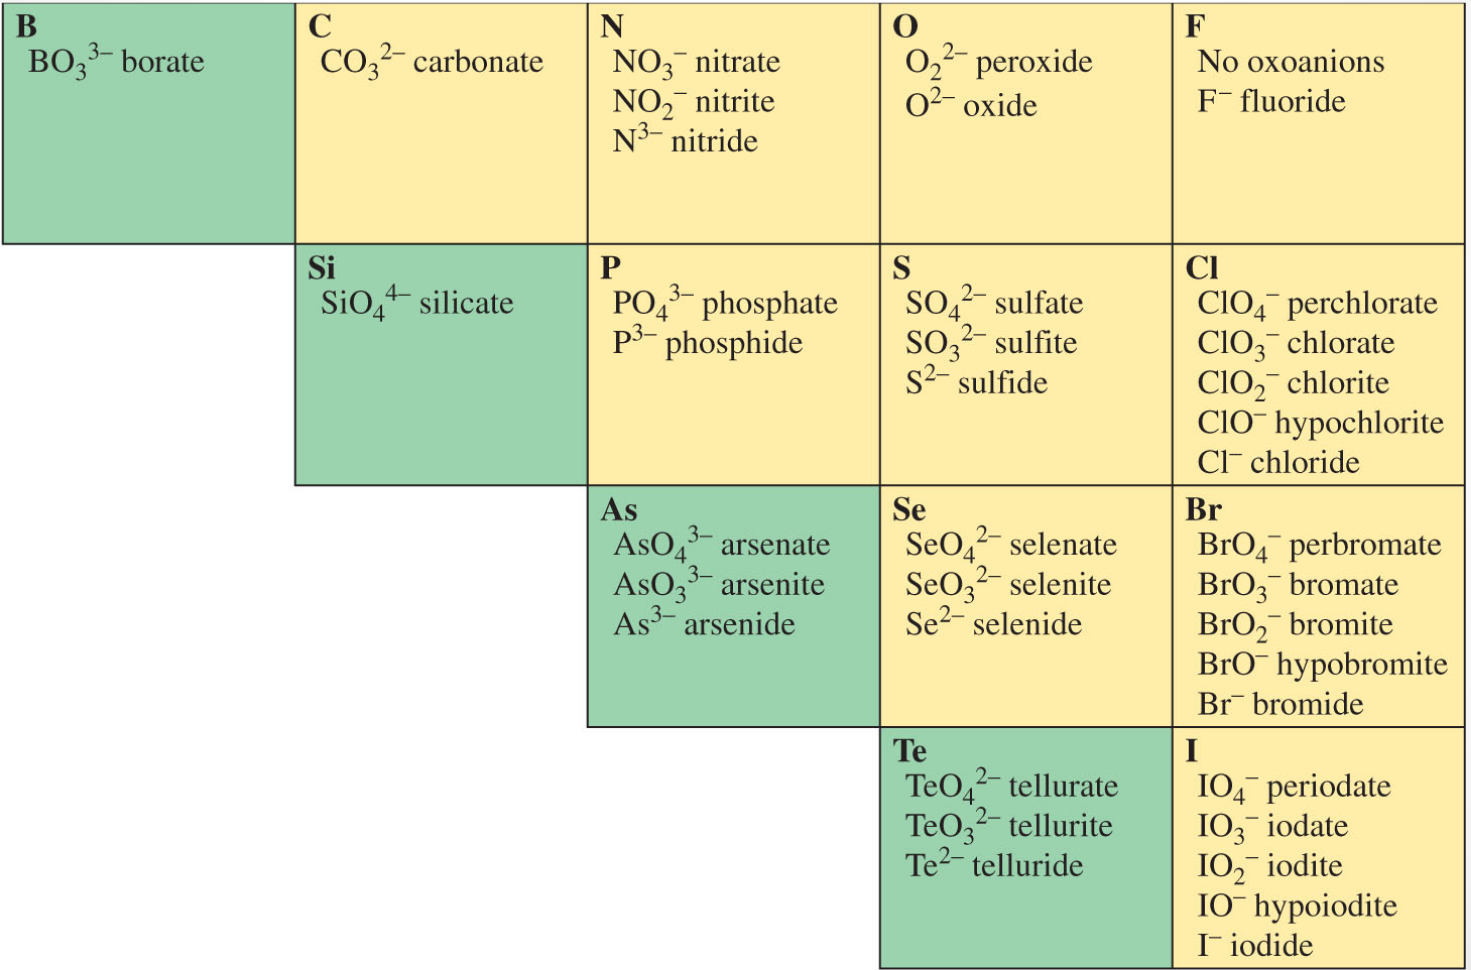
\includegraphics[width=\linewidth]{polyatomic_ion}
\end{frame}

\begin{frame}{Additional Polyatomic Ions}
  \centering
  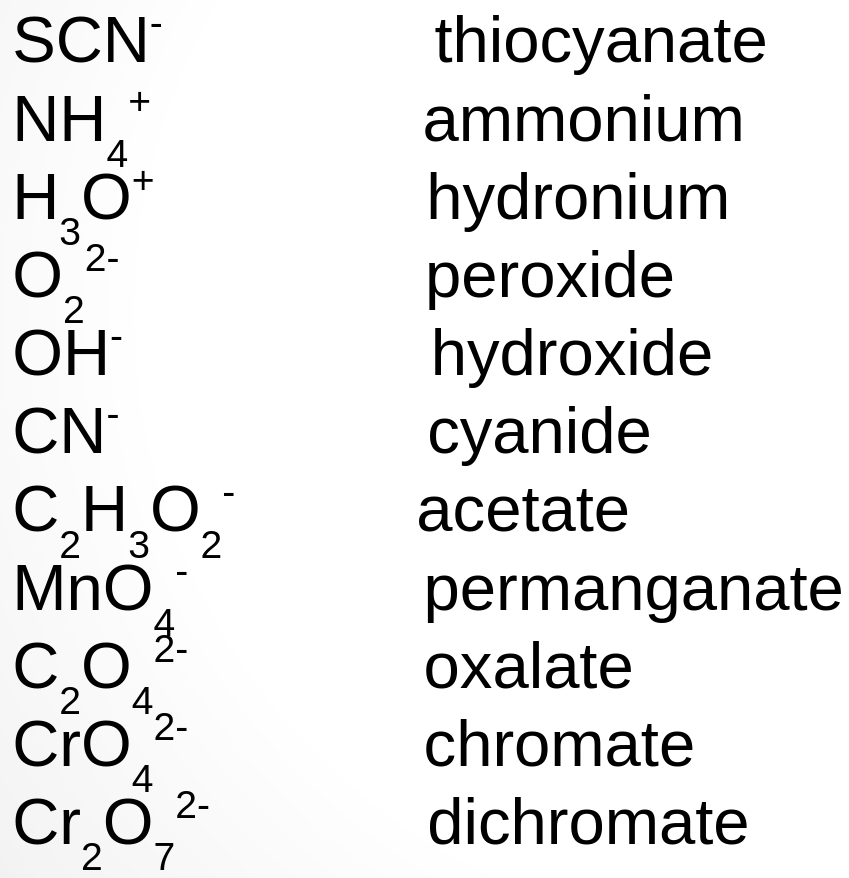
\includegraphics[width=0.7\linewidth]{more_poly_ions}
\end{frame}

\subsection{Formulas for Ionic Compounds}

\begin{frame}{Molecular Formulas for Ionic Compounds}
  The sum of the cations and anions equals to zero. The
  cation is written first then anion.

  \textbf{Examples:} Practice determining the oxidation states
  \begin{itemize}
  \item CaCO$_3$
  \item BaCl$_2$
  \item FeCl$_3$
  \item Ca(NO$_3$)$_2$
  \end{itemize}
\end{frame}

\section{Naming and Writing Formulas}

\subsection{Ionic Compounds}

\begin{frame}{Naming Ions}
  \textbf{Metals} - start with the element and end with ion

  \centering
  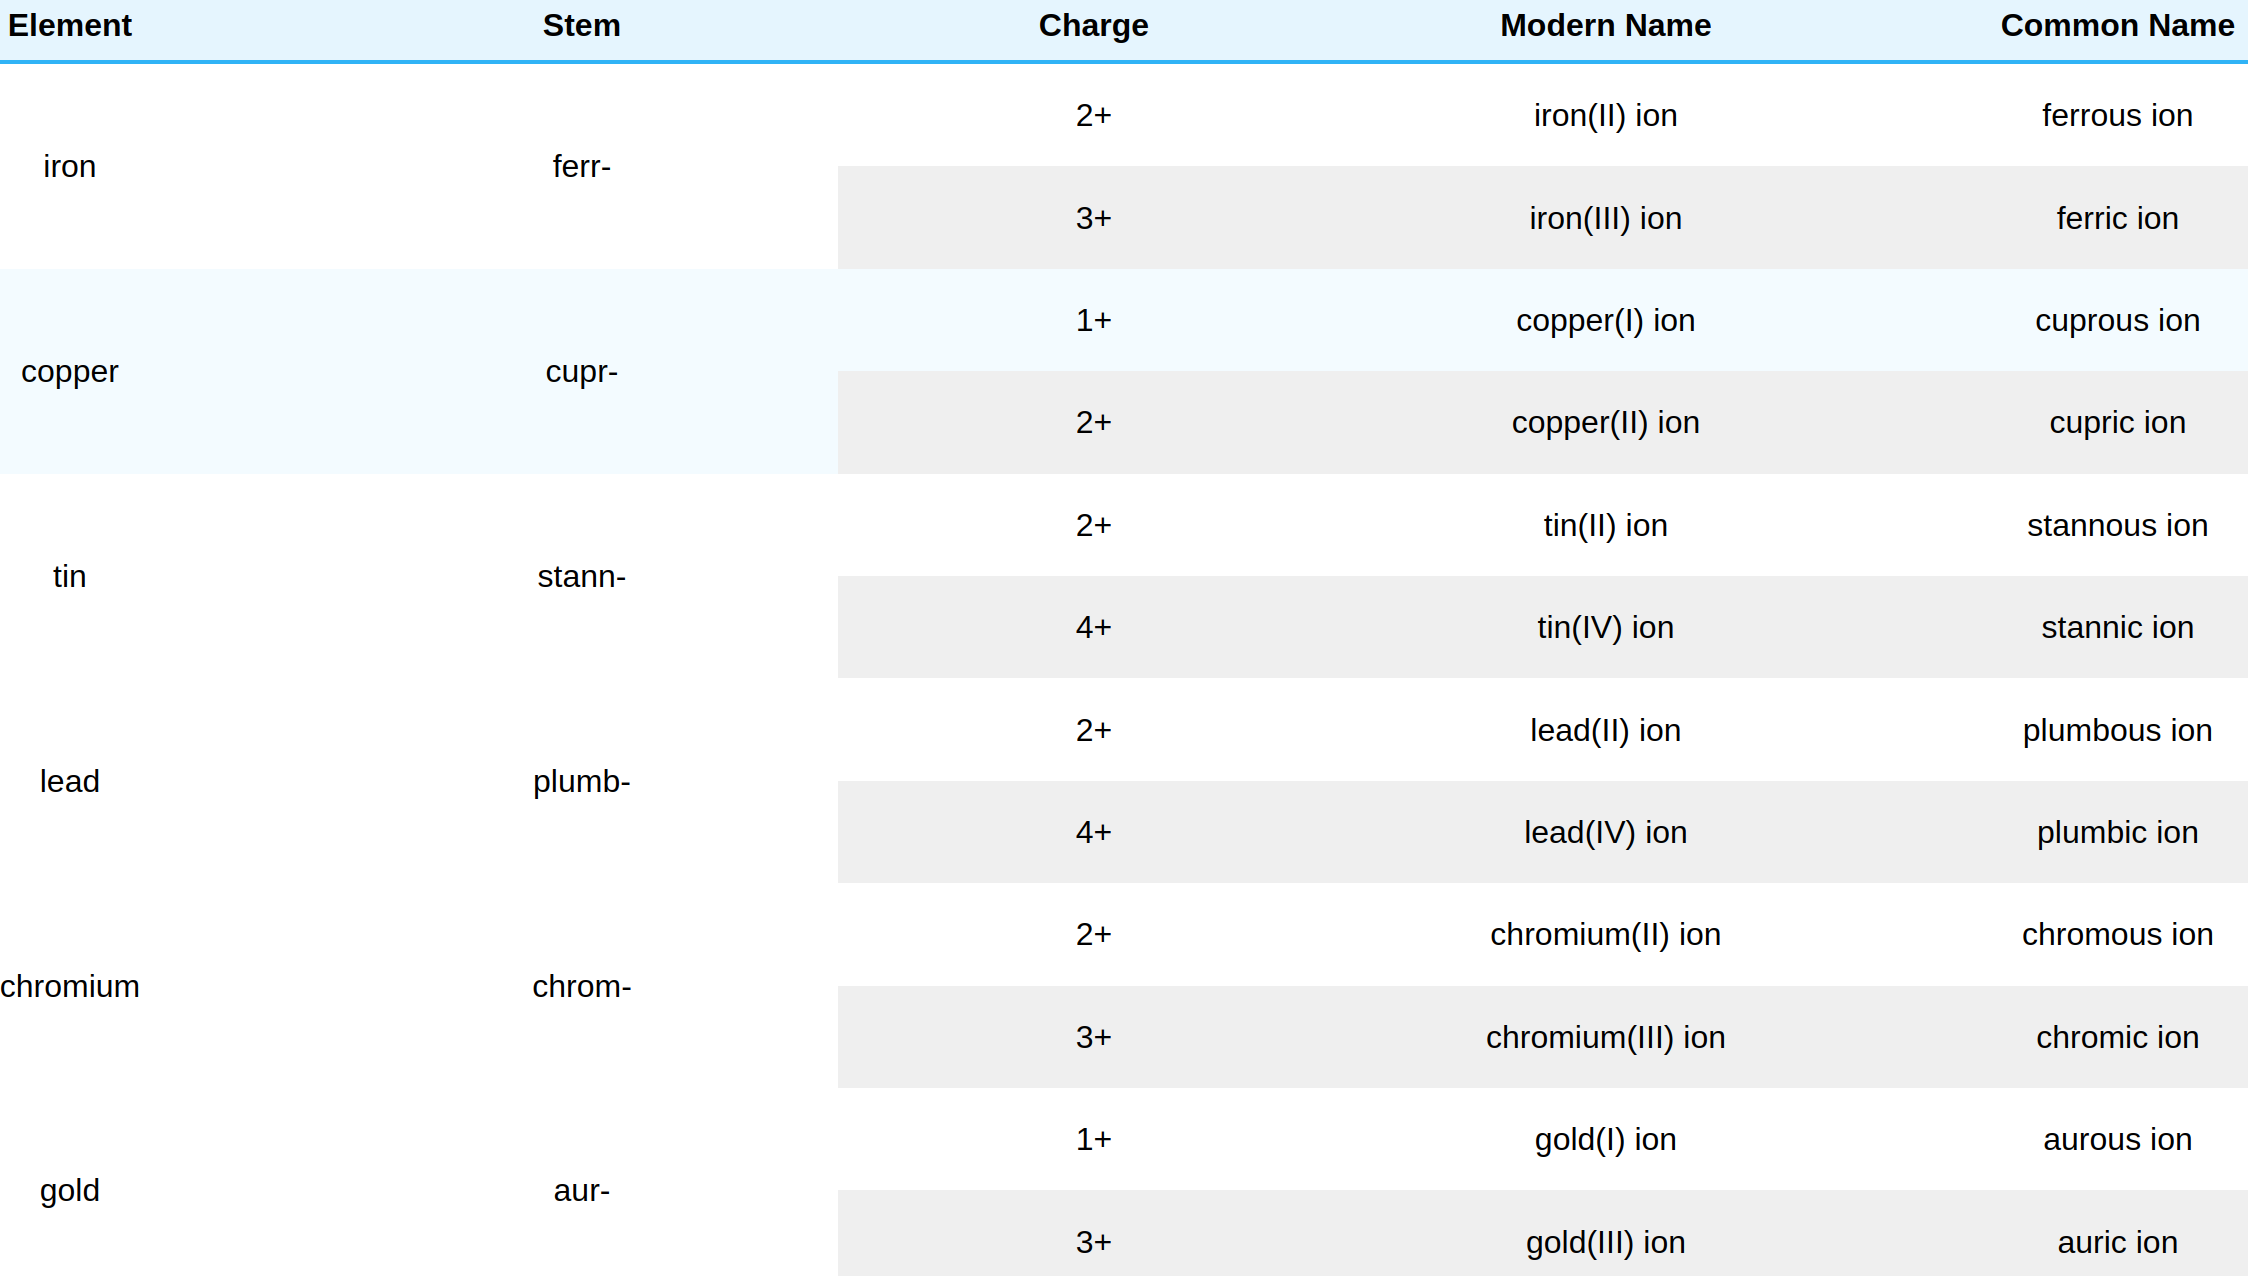
\includegraphics[width=\linewidth]{ions_names}
\end{frame}

\begin{frame}{Naming Nonmetal Ions}
  \textbf{Nonmetals} - replace suffix with -ide and end with ion

  \centering
  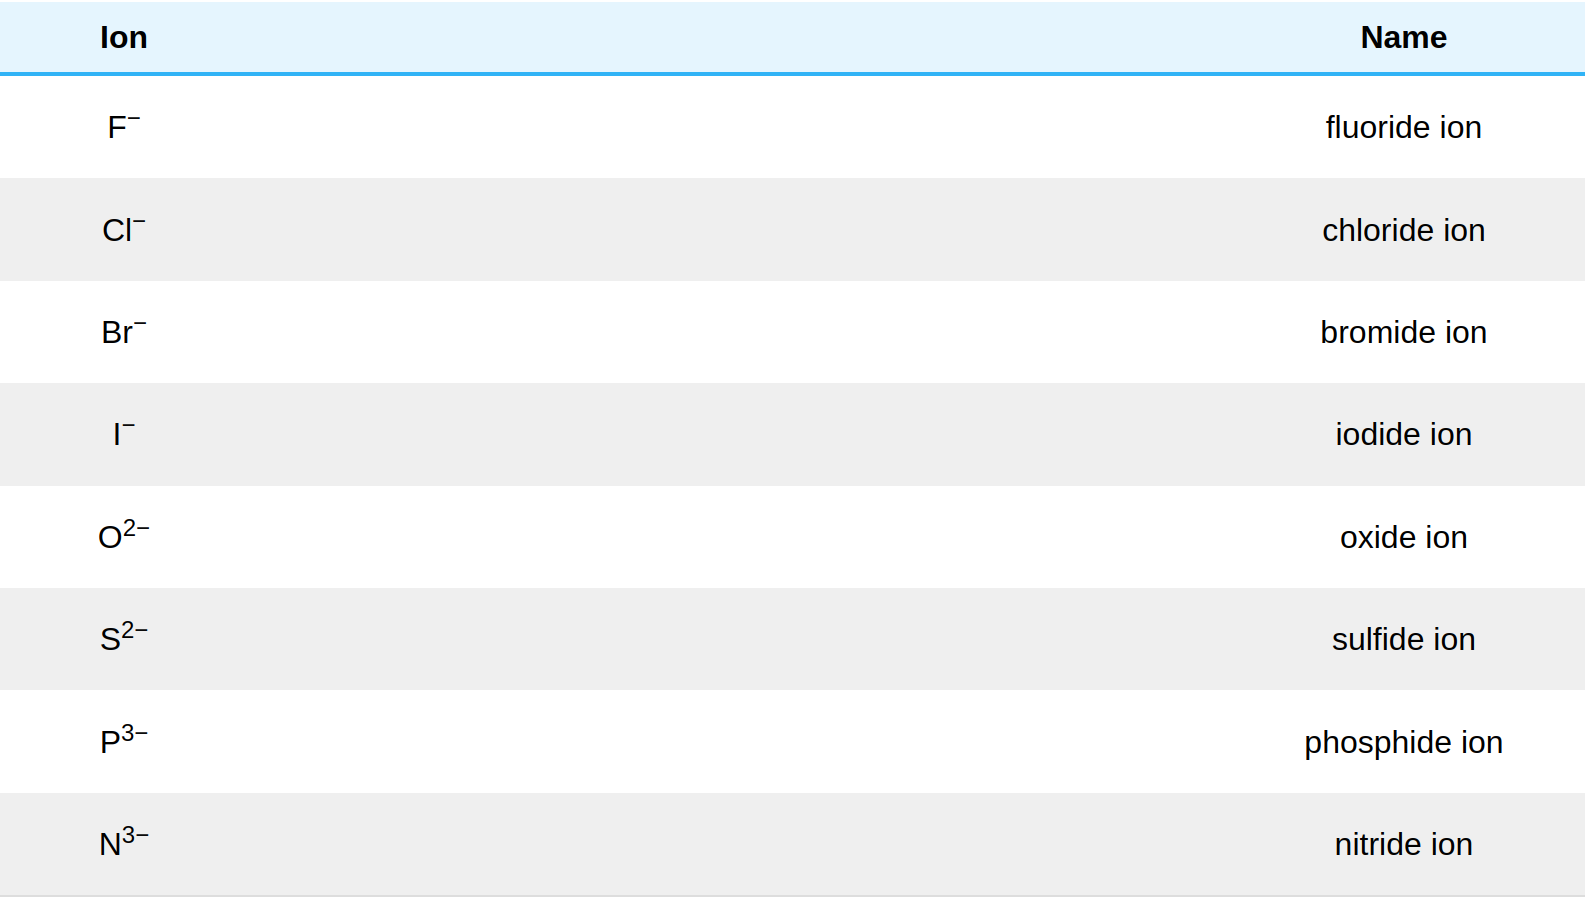
\includegraphics[width=\linewidth]{nonmetal_ions}
\end{frame}

\begin{frame}{Practice: Name Each Ion}
  \begin{itemize}
  \item Fe$^{2+}$
  \item F$^-$
  \item Ba$^+$
  \item S$^{2-}$
  \end{itemize}
\end{frame}

\begin{frame}{Naming Binary Ionic Compounds}
  The metal cation is named first, followed by the nonmetal anion.
  The word ion is dropped from both parts.

  \centering
  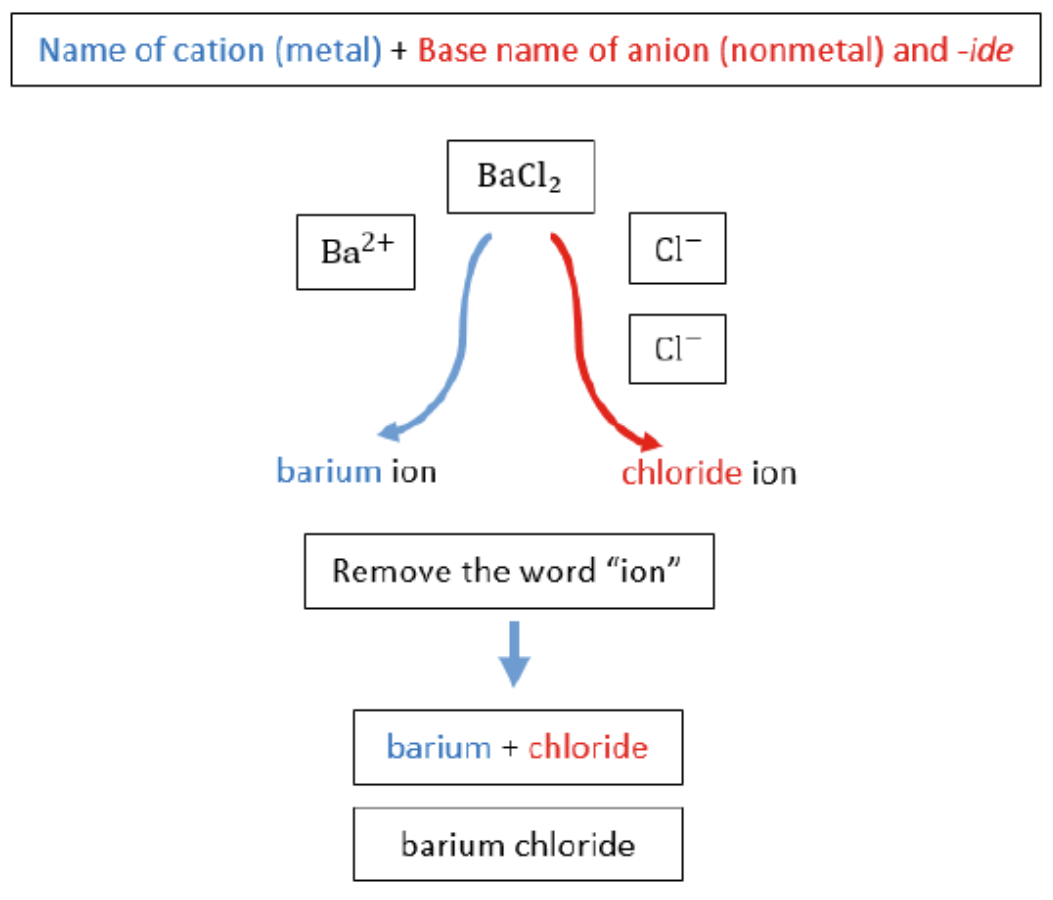
\includegraphics[width=0.7\linewidth]{barium_examp.png}
\end{frame}

\begin{frame}{Practice: Name the Ionic Compound}
  \begin{itemize}
  \item CaCl$_2$
  \item Ca$_3$P$_2$
  \item MgO
  \item FeCl$_2$
  \item Co$_2$O$_3$
  \end{itemize}
\end{frame}

\subsection{Molecular Compounds}

\begin{frame}{Naming Molecular Compounds}
  \begin{center}
    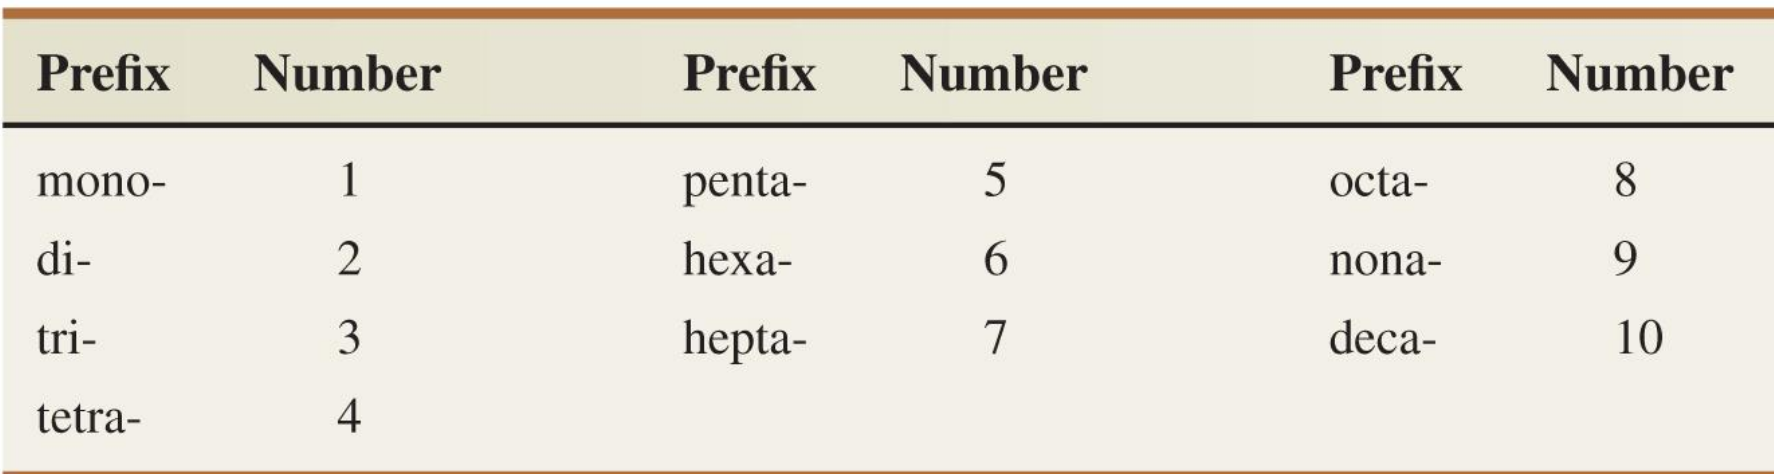
\includegraphics[width=\linewidth]{prefix_name}
  \end{center}
  
  \begin{enumerate}
  \item Use numerical prefix for the element (usually ignore the first
    when using ``mono'')
  \item Add ``-ide'' to the second element
  \end{enumerate}
\end{frame}

\begin{frame}{Naming Binary Molecular Compounds}
  \begin{itemize}
  \item H$_2$O
  \item N$_2$O$_4$
  \item CO
  \item CH$_4$
  \end{itemize}
\end{frame}

\subsection{Acids and Bases}

\begin{frame}{Naming Acids and Bases}
  \begin{center}
    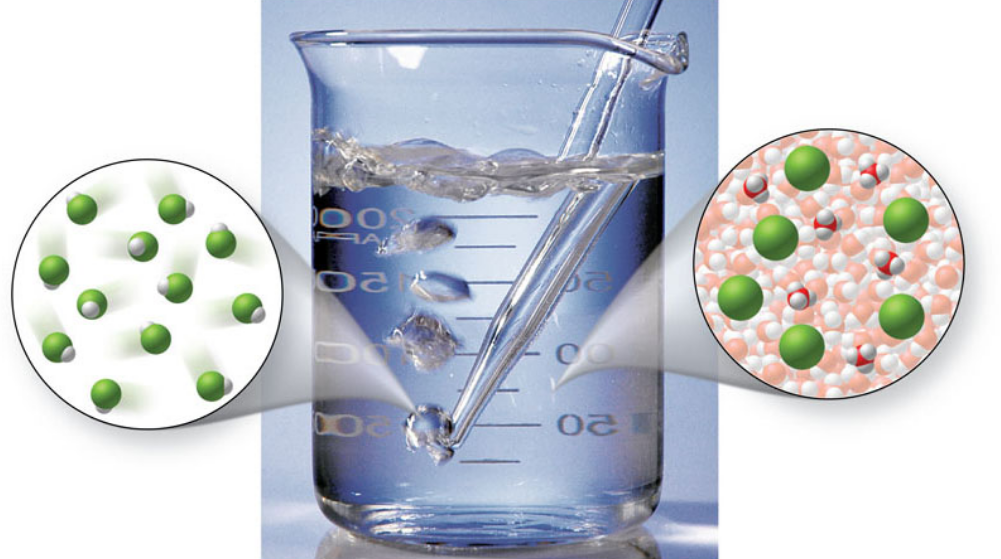
\includegraphics[width=0.5\linewidth]{acid_base}
  \end{center}

  \begin{enumerate}
  \item If anion ends in ``-ide,'' add ``hydro'' before the
    root of the anion name followed by ``-ic acid''
  \item If anion ends in ``-ate,'' use the root of the anion
    name followed by ``-ic acid''
  \item If anion ends in ``-ite,'' use the root of the anion
    name followed by ``-ous acid''
  \end{enumerate}
\end{frame}

\begin{frame}{Practice: Naming the Acid}
  \begin{itemize}
  \item HCl
  \item HNO$_3$
  \item H$_2$CO$_3$
  \item H$_2$SO$_3$
  \end{itemize}
\end{frame}

\end{document}
